\subsection{Distances}

$$ d(p,q) = {\sqrt {(q.x-p.x)^{2}+(q.y-p_.y)^{2}}} $$

$$ d(p,q) |p.x - q.x| + |p.y - q.y| $$

\subsection{Maximum possible Manhattan distance between two points given n points}

Given n points, for instance:
\begin{center}
  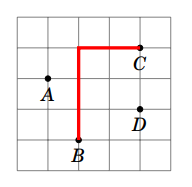
\includegraphics[scale=.6, keepaspectratio]{./theoretical/img/manhattan_before.png}
\end{center}

Rotate all coordinates $45^{o}$ do that $(x, y)$ becomes $(x+y, y-x)$, so, $p$ becomes $p'$ and $q$ becomes $q'$.
\begin{center}
  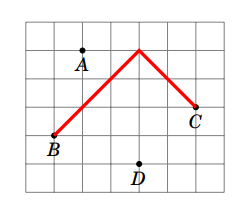
\includegraphics[scale=.6, keepaspectratio]{./theoretical/img/manhattan_after.png}
\end{center}

The maximum manhattan distance is obtaining by choosing the two points that maximize:

$$ max(|p'.x - q'.x|, |p'.y - q'.y|) $$